\documentclass[10pt,twocolumn]{article}

\usepackage[margin=0.75in]{geometry}
\usepackage[T1]{fontenc}
\usepackage{lmodern}
\usepackage{microtype}
\usepackage{amsmath,amssymb,amsfonts}
\usepackage{graphicx}
\usepackage{booktabs}
\usepackage[numbers]{natbib}
\usepackage{hyperref}
\usepackage{url}
\usepackage{float}
\usepackage{xcolor}
\usepackage{enumitem}

\setlength{\columnsep}{0.25in}
\setlength{\parskip}{0.45em}
\setlength{\parindent}{0pt}
\setlength{\textfloatsep}{10pt plus 2pt minus 2pt}
\setlength{\floatsep}{8pt plus 2pt minus 2pt}
\setlength{\intextsep}{8pt plus 2pt minus 2pt}
\linespread{1.03}

\hypersetup{
    colorlinks=true,
    citecolor=blue,
    linkcolor=blue,
    urlcolor=blue
}

\title{\textbf{Racketlon Match Prediction using Dynamic Ratings and Machine Learning Models}}

\author{
Zain Magdon-Ismail \\
Rensselaer Polytechnic Institute
}

\date{}

\begin{document}

\twocolumn[
    \maketitle
    \begin{abstract}
        Racketlon is a multi-sport competition in which two players compete sequentially across table tennis, badminton, squash, and tennis, with the winner determined by total points accumulated across all four sports. Predicting outcomes in this setting is challenging because player skill is both sport-specific and temporally dynamic, and because match-level outcomes must be assembled from structured sport-level predictions. In this work, I develop an end-to-end machine learning pipeline for Racketlon match prediction, beginning with automated data collection and cleaning, continuing through leakage-safe feature engineering and dynamic rating estimation, and culminating in a comparison of predictive models of increasing complexity. The evaluated approaches include a historical-average benchmark, ridge regression, a neural network with learned player embeddings, and a gradient boosted tree model. Across these experiments, the strongest overall finding is that carefully designed domain-specific features provide the majority of the predictive signal. The best-performing model is a gradient boosted tree ensemble with a match-level mean absolute error of 13.89 and winner accuracy of 73.4\%, but the gain over simpler feature-based models is modest. This suggests that representation design is at least as important as model complexity in structured sports prediction problems. A secondary KD-tree-based confidence experiment is also included in the appendix, where geometric neighborhood statistics are tested as potential proxies for uncertainty.
    \end{abstract}
    \vspace{0.35cm}
]

% =========================================================
\section{Introduction}

Racketlon presents a distinctive and challenging prediction task in sports analytics. Unlike standard single-sport forecasting problems, each Racketlon match is composed of four separate disciplines played in sequence: table tennis (TT), badminton (BD), squash (SQ), and tennis (TN). The final winner is not determined by winning a majority of sports, but by accumulating the highest total number of points across all four. As a result, successful prediction requires reasoning simultaneously about sport-specific skill, cross-sport complementarity, short-term form, and aggregate score composition.

This structure introduces several modeling challenges. First, player ability is inherently multi-dimensional. A player may be dominant in badminton but weak in table tennis, or broadly balanced but without a major advantage in any single discipline. Second, player strength is not static: performance changes over time due to experience, inactivity, improvement, decline, and matchup context. Third, the final prediction target is itself hierarchical. A full match prediction is assembled from multiple sport-level score predictions, which must then be aggregated into a final total margin and winner.

The goal of this project is to build a complete predictive pipeline for Racketlon match outcomes. This includes data acquisition, cleaning, feature engineering, dynamic rating estimation, model training, evaluation, and deployable inference. Rather than treating the task as a black-box classification problem, I formulate it as a structured regression problem in which sport-level score differences and totals are predicted first, then decoded into realistic scorelines and aggregated into final match outcomes.

A second motivation of the project is methodological. I compare multiple models of increasing complexity in order to study how much performance comes from model flexibility versus feature design. In particular, I evaluate a simple historical-average benchmark, a regularized linear model, a player embedding neural network, and a gradient boosted tree system. This progression makes it possible to answer a key question: in a structured prediction problem like this one, where is the real source of performance gain?

The final conclusion is that feature engineering plays the dominant role. More expressive models do improve performance, but only slightly once the feature representation becomes sufficiently informative. This observation is central to the project and, more broadly, illustrates an important principle in applied machine learning: when structure is known, encoding it explicitly can be more valuable than increasing raw model complexity.

% =========================================================
\section{Problem Formulation}

Let the four sports be indexed by
\[
    s \in \{TT, BD, SQ, TN\}.
\]
For a match between players $p_1$ and $p_2$, let $y^{(s)}_{p1}$ and $y^{(s)}_{p2}$ denote the points won by each player in sport $s$.

The project predicts two sport-level regression targets for each discipline:
\[
    y^{(s)}_{\text{diff}} = y^{(s)}_{p1} - y^{(s)}_{p2},
\]
\[
    y^{(s)}_{\text{total}} = y^{(s)}_{p1} + y^{(s)}_{p2}.
\]

From these sport-level quantities, a match-level total difference is formed:
\[
    y_{\text{match diff}} = \sum_s y^{(s)}_{\text{diff}}.
\]

The winner label is then induced by the sign of the total match difference:
\[
    y_{\text{winner}} =
    \begin{cases}
        1 & \text{if } y_{\text{match diff}} > 0, \\
        0 & \text{otherwise.}
    \end{cases}
\]

This formulation is preferable to directly predicting only the winner, because it preserves much more structure. Predicting score differentials and totals provides several advantages:
\begin{enumerate}[leftmargin=1.2em,itemsep=0.25em]
    \item it supports winner prediction as a downstream consequence rather than a single opaque label,
    \item it enables realistic sport-level score reconstruction,
    \item it produces interpretable diagnostics at the sport level,
    \item it allows evaluation of both margin prediction and classification accuracy.
\end{enumerate}

Thus, the project treats Racketlon as a structured regression problem with a derived classification output.

% =========================================================
\section{Related Work}

This project draws on three primary areas of prior work: rating systems for competitive skill, supervised learning for structured data, and representation learning. In addition, we briefly consider work on confidence estimation in predictive models.

\subsection{Rating Systems and Skill Modeling}

Classical rating systems such as Elo \citep{elo1978} provide a principled framework for modeling player skill through pairwise competition. These systems are attractive because they are interpretable, sequentially updatable, and robust to sparse data. However, standard Elo formulations are primarily designed for win/loss outcomes and do not directly incorporate score margins.

In sports where score differentials provide additional signal, extensions to Elo incorporate margin-of-victory information and nonlinear mappings between skill difference and outcome. This motivates the dynamic rating system used in this work, which maps rating differences to expected score differences using a bounded nonlinear transformation. This formulation better reflects the constraints of Racketlon scoring, where outcomes are naturally limited by the rules of each sport.

\subsection{Machine Learning for Tabular Data}

Structured prediction problems with engineered features are commonly addressed using linear models and tree-based ensembles. Regularized linear models provide a simple and interpretable baseline by learning additive relationships between features. However, they cannot capture interactions between features or nonlinear effects.

Gradient boosting \citep{friedman2001} is widely regarded as one of the most effective approaches for tabular data. Modern implementations such as XGBoost \citep{chen2016xgboost} and LightGBM \citep{ke2017lightgbm} construct ensembles of decision trees that can model threshold effects and complex feature interactions. This motivates the use of boosted trees as the final model in this project, particularly given the structured and heterogeneous nature of the feature set.

\subsection{Representation Learning and Player Embeddings}

Embedding-based models provide a way to learn latent representations of entities such as players. These approaches are widely used in recommender systems and natural language processing \citep{koren2009matrix, mikolov2013word2vec}, where they capture similarity relationships that are not explicitly encoded in the input features.

In this project, player embeddings are used to model latent aspects of player skill and interaction effects. While this approach is flexible, prior work has shown that neural networks do not always outperform simpler models on structured tabular data. This motivates evaluating embedding models alongside linear and tree-based approaches rather than assuming their superiority.

\subsection{Confidence and Uncertainty Estimation}

In addition to predictive accuracy, it is often desirable to estimate the confidence or reliability of predictions. Classical approaches include probabilistic models, Bayesian methods, and ensemble-based uncertainty estimation. In non-parametric settings, nearest-neighbor methods \citep{cover1967} use local neighborhood structure as a proxy for confidence, under the assumption that similar inputs yield similar outputs.

KD-trees \citep{bentley1975} provide an efficient data structure for nearest-neighbor search and are commonly used to analyze local geometry in feature space. In this work, KD-trees are used in a secondary experiment to test whether local density and outcome consistency correlate with prediction error. This experiment provides insight into the relationship between geometric similarity and model uncertainty in structured prediction problems.

% =========================================================
\section{Data Collection and Cleaning}

The dataset was constructed from historical Racketlon match records scraped from tournament websites. The scraping stage required handling nonuniform page layouts and extracting structured sport-level results from raw web pages. After collection, the raw data was cleaned to remove malformed entries, incomplete results, and matches unsuitable for analysis.

A central preprocessing step was \textbf{name normalization}. Because all historical statistics depend on consistent player identity, player names were standardized to lowercase strings with cleaned formatting. This was necessary to ensure that repeated appearances by the same player were aggregated correctly.

Invalid rows were removed when score information was incomplete or clearly inconsistent with a valid four-sport Racketlon match. The cleaned dataset was then chronologically ordered using available match date and time fields, since the feature pipeline depends on sequential processing.

Although the project ultimately trains on a single primary dataset, substantial transformation is performed between the raw scraped data and the final training matrix. In practice, the workflow produces multiple stages of data representation:
\begin{enumerate}[leftmargin=1.2em,itemsep=0.25em]
    \item raw scraped match records,
    \item cleaned match-level results,
    \item leakage-safe engineered feature tables,
    \item serialized inference state for future predictions.
\end{enumerate}

This staged pipeline is important for reproducibility and mirrors real machine learning workflows more closely than a single static CSV.

% =========================================================
\section{Feature Engineering}

Feature engineering is one of the most important components of the project. All features were constructed \emph{chronologically}: for a given match, only information available before that match was used. This prevents target leakage and makes offline evaluation consistent with real-world deployment.

The final feature space captures several complementary views of player performance.

\subsection{Rating-Based Features}

The rating system produces one scalar rating per player per sport. Differences in these ratings provide a direct estimate of relative skill:
\[
    \text{rating diff}^{(s)} = R^{(s)}_{p1} - R^{(s)}_{p2}.
\]
These features are among the most predictive in the final model.

\subsection{Recent Form}

Recent-form features summarize short-term performance over rolling windows. These include recent mean score difference, recent residual mean, volatility, and momentum. For example, a momentum feature compares short-window and longer-window performance:
\[
    \text{momentum}^{(s)}_{5,20}
    =
    \text{mean diff}^{(s)}_{5}
    -
    \text{mean diff}^{(s)}_{20}.
\]
Such features allow the model to detect players who are improving or declining more quickly than the long-term rating system alone would suggest.

\subsection{Residual Performance}

Residuals are defined as actual score difference minus expected score difference under the rating model. They quantify over-performance or under-performance relative to rating-based expectation:
\[
    \text{residual} = d - \hat d.
\]
This provides a way to distinguish players whose results are systematically stronger or weaker than their current ratings imply.

\subsection{Long-Term Aggregates}

In addition to recent windows, long-term averages are computed using historical records. These include shrunk averages of score difference, total points, and win rate. Such features stabilize estimates for players with smaller sample sizes and help distinguish players with similar short-term form but different historical baselines.

\subsection{Head-to-Head Features}

Matchup-specific information is captured through head-to-head statistics. These include prior meetings, average margin between the players, and head-to-head win rate. Both overall and sport-specific versions are maintained.

\subsection{Why the Feature Set Matters}

Taken together, these features provide a multi-timescale representation of player strength. The rating system captures broad sport-specific skill, recent-form features capture short-term fluctuations, residual statistics capture deviation from expectation, and head-to-head features capture matchup effects.

A key insight of the project is that this feature set already encodes substantial nonlinear structure. For example, the rating-to-score mapping is nonlinear, recent residual behavior measures deviations from a nonlinear expectation, and head-to-head effects introduce interaction-specific corrections. As a result, even comparatively simple models receive highly informative inputs.

% =========================================================
\section{Dynamic Rating Model}

Each player is assigned one rating per sport:
\[
    R_{p,TT}, \quad R_{p,BD}, \quad R_{p,SQ}, \quad R_{p,TN}.
\]

These ratings are not interpreted as probabilities of winning. Instead, they are mapped directly to an expected sport-level score difference.

\subsection{Rating-to-Score Mapping}

Let $x = R_1 - R_2$ be the rating difference in a given sport. The expected score difference is modeled as
\[
    \hat{d} = 21 \tanh\left(\frac{\alpha x}{2}\right),
\]
where $\alpha$ is sport-specific.

This mapping is important for several reasons:
\begin{enumerate}[leftmargin=1.2em,itemsep=0.25em]
    \item it is bounded between $-21$ and $21$, which is consistent with realistic score margins,
    \item it is approximately linear near zero, so small rating differences remain interpretable,
    \item it saturates for large rating differences, reflecting the fact that scores cannot increase without bound.
\end{enumerate}

In other words, the relationship between skill difference and score difference is inherently nonlinear. If one player is slightly stronger, the model expects a modest margin. If one player is much stronger, the predicted score difference increases, but eventually flattens because sport scores are bounded. This provides a principled reason to incorporate nonlinearity even before any machine learning model is trained.

\subsection{Experience-Dependent Learning Rate}

The rating update step uses a learning rate that depends on player experience:
\[
    \eta(g)
    =
    \eta_{\min}
    +
    (\eta_{\max}-\eta_{\min}) e^{-g/\tau},
\]
where $g$ is the number of prior matches in that sport. This allows the rating to move quickly for players with little data and stabilize as more evidence accumulates.

\subsection{Time-Based Adaptation}

To make the system more responsive after long inactivity, a time multiplier is used:
\[
    t_{\mathrm{mult}}
    =
    1 + c_s \left(1 - e^{-d/\tau_s}\right),
\]
where $d$ is days since last match in that sport. This increases update sensitivity after layoffs without explicitly decaying stored ratings.

\subsection{Update Rule}

A simplified update rule is
\[
    \text{step} = \eta \cdot t_{\mathrm{mult}} \cdot (d - \hat d),
\]
followed by a symmetric update to the two players’ ratings. Conceptually, this means that ratings change in proportion to prediction error, scaled by experience and inactivity.

The rating system serves a dual role in the project. It is both an interpretable standalone estimate of player skill and a powerful feature generator for downstream supervised models.

% =========================================================
\section{Models}

The project evaluates a progression of models of increasing complexity. This progression is designed not only to improve performance, but also to answer a methodological question: how much additional value do more expressive models provide once the feature space is already strong?

\subsection{Historical-Average Baseline}

The simplest benchmark predicts sport-level score difference using player historical averages:
\[
    \hat d^{(s)} = \bar d_{p1}^{(s)} - \bar d_{p2}^{(s)}.
\]
This model is transparent and fast. It uses only prior average performance and provides a genuine lower bound on performance.

Its main limitation is that it cannot adapt well to short-term form, nonlinear effects, or richer interaction patterns. It also treats historical evidence too uniformly relative to more structured models.

\subsection{Linear Model}

The first feature-based model is ridge regression, which predicts
\[
    \hat y = w^T x + b.
\]
Here, $x$ is the engineered feature vector, $w$ is the learned weight vector, and $b$ is the intercept.

In this project, $w^T x + b$ corresponds to a weighted combination of features such as:
\begin{itemize}[leftmargin=1.2em,itemsep=0.25em]
    \item rating differences,
    \item recent-form statistics,
    \item long-term aggregates,
    \item head-to-head statistics.
\end{itemize}

This model is strong because the feature set is already informative. However, it is limited to additive effects and cannot represent interactions such as ``recent form matters more when rating difference is small'' or ``head-to-head matters differently for different sports.''

\subsection{Player Embedding Model}

To introduce learned latent structure, I trained a PyTorch-based neural model with player embeddings. Each player $p$ is assigned a learned vector
\[
    e_p \in \mathbb{R}^{16}.
\]

For players $p_1$ and $p_2$, the model forms a combined input:
\[
    [e_1, e_2, e_1 - e_2, e_1 \odot e_2, x_{\text{num}}],
\]
where $x_{\text{num}}$ denotes the numeric engineered features, and $\odot$ is elementwise multiplication.

This input is passed through a multilayer perceptron with two hidden layers:
\[
    \text{input} \rightarrow 128 \rightarrow 64 \rightarrow 2,
\]
with ReLU activations and dropout between hidden layers. The two outputs correspond to predicted sport difference and predicted sport total.

This architecture is expressive enough to learn latent similarities between players and nonlinear combinations of embedding interactions and handcrafted features. However, in practice it performs very similarly to the linear model, indicating that the feature space already captures most of the useful structure.

\subsection{Gradient Boosted Trees}

The final model is a gradient boosted tree system (implemented via CatBoost) trained separately by sport. For each sport, three regressors are used:
\begin{enumerate}[leftmargin=1.2em,itemsep=0.25em]
    \item a base differential model,
    \item a residual correction model,
    \item a total-points model.
\end{enumerate}

The final sport differential prediction is
\[
    \hat d = b + 0.7r,
\]
where $b$ is the base prediction and $r$ is the residual correction.

This architecture allows the model to first learn broad, stable skill-gap structure and then refine its prediction using residual patterns. The tree-based formulation is especially useful for capturing threshold effects and nonlinear interactions. For example, the effect of head-to-head history may depend on rating gap, and recent form may matter more in close matches than in highly asymmetric ones. Finally, the raw continuous outputs for total points and point differentials are decoded back into legal, sport-specific scorelines (e.g., forcing a 21-point game format for the first three sports).

Even so, the improvement over simpler feature-based models is modest. This result is important: it suggests that the feature engineering pipeline already explains much of the structure that more flexible models would otherwise need to discover.

% =========================================================
\section{Experimental Setup}

The dataset was ordered chronologically and split into training and test portions using a forward split. This better reflects real-world prediction than random shuffling, since future matches should be predicted using only past information.

The primary match-level evaluation metrics are:
\begin{itemize}[leftmargin=1.2em,itemsep=0.25em]
    \item \textbf{Mean Absolute Error (MAE)} on total match score difference,
    \item \textbf{Winner accuracy} derived from the sign of predicted match difference.
\end{itemize}

These metrics complement one another. MAE measures quality of margin prediction, while winner accuracy measures practical classification performance. In general, winner accuracy is easier to optimize than exact score-difference prediction, since predicting the correct sign requires less precision than predicting the exact margin.

% =========================================================
\section{Results}

The final boosted-tree model achieves the strongest overall match-level performance among the models considered, with mean absolute error 13.89 and winner accuracy 73.4\%. Figure~\ref{fig:scatter} shows predicted versus actual total match score difference, and Figure~\ref{fig:cm} shows the winner confusion matrix.

Table~\ref{tab:results} details the match-level evaluation metrics across all tested models, and Table~\ref{tab:sport_results} breaks down the mean absolute error for point differentials and total points by sport.

\begin{table}[H]
    \centering
    \caption{Match-Level Performance Comparison}
    \label{tab:results}
    \begin{tabular}{lcc}
        \toprule
        Model            & Match MAE & Accuracy \\
        \midrule
        Baseline         & 16.70     & 66.0\%   \\
        Linear (Ridge)   & 14.05     & 73.3\%   \\
        Player Embedding & 14.00     & 72.8\%   \\
        Boosted Trees    & 13.89     & 73.4\%   \\
        \bottomrule
    \end{tabular}
\end{table}

\begin{table*}[t]
    \centering
    \caption{Sport-Level Mean Absolute Error (MAE) for Difference and Total Points}
    \label{tab:sport_results}
    \begin{tabular}{lcccccccc}
        \toprule
                         & \multicolumn{2}{c}{Table Tennis (TT)} & \multicolumn{2}{c}{Badminton (BD)} & \multicolumn{2}{c}{Squash (SQ)} & \multicolumn{2}{c}{Tennis (TN)}                               \\
        \cmidrule(lr){2-3} \cmidrule(lr){4-5} \cmidrule(lr){6-7} \cmidrule(lr){8-9}
        Model            & Diff                                  & Total                              & Diff                            & Total                           & Diff & Total & Diff & Total \\
        \midrule
        Baseline         & 6.87                                  & 8.94                               & 7.50                            & 8.68                            & 8.15 & 8.53  & 5.51 & 9.72  \\
        Linear (Ridge)   & 6.04                                  & 4.69                               & 6.51                            & 4.64                            & 7.06 & 4.84  & 5.42 & 8.88  \\
        Player Embedding & 5.96                                  & 4.69                               & 6.33                            & 4.75                            & 6.97 & 5.11  & 5.47 & 9.23  \\
        Boosted Trees    & 5.93                                  & 4.02                               & 6.30                            & 3.97                            & 6.94 & 4.32  & 5.52 & 8.96  \\
        \bottomrule
    \end{tabular}
\end{table*}

\begin{figure}[H]
    \centering
    
\includegraphics[width=0.92\columnwidth]{figures/match_total_diff_scatter.png}
    \caption{Predicted versus actual total match score difference for the final boosted-tree model.}
    \label{fig:scatter}
\end{figure}

\begin{figure}[H]
    \centering
    
\includegraphics[width=0.82\columnwidth]{figures/winner_confusion_matrix.png}
    \caption{Winner prediction confusion matrix for the final model.}
    \label{fig:cm}
\end{figure}

The scatter plot shows that the model captures the overall trend in match score difference, though prediction spread increases for more extreme outcomes. This is expected: close matches are often easier to place near the correct region, while large margins are harder to estimate precisely. The confusion matrix indicates that winner prediction is substantially more reliable than exact score-margin prediction.

To compare models directly, Figures~\ref{fig:model_mae} and \ref{fig:model_acc} summarize performance across all approaches.

\begin{figure}[H]
    \centering
    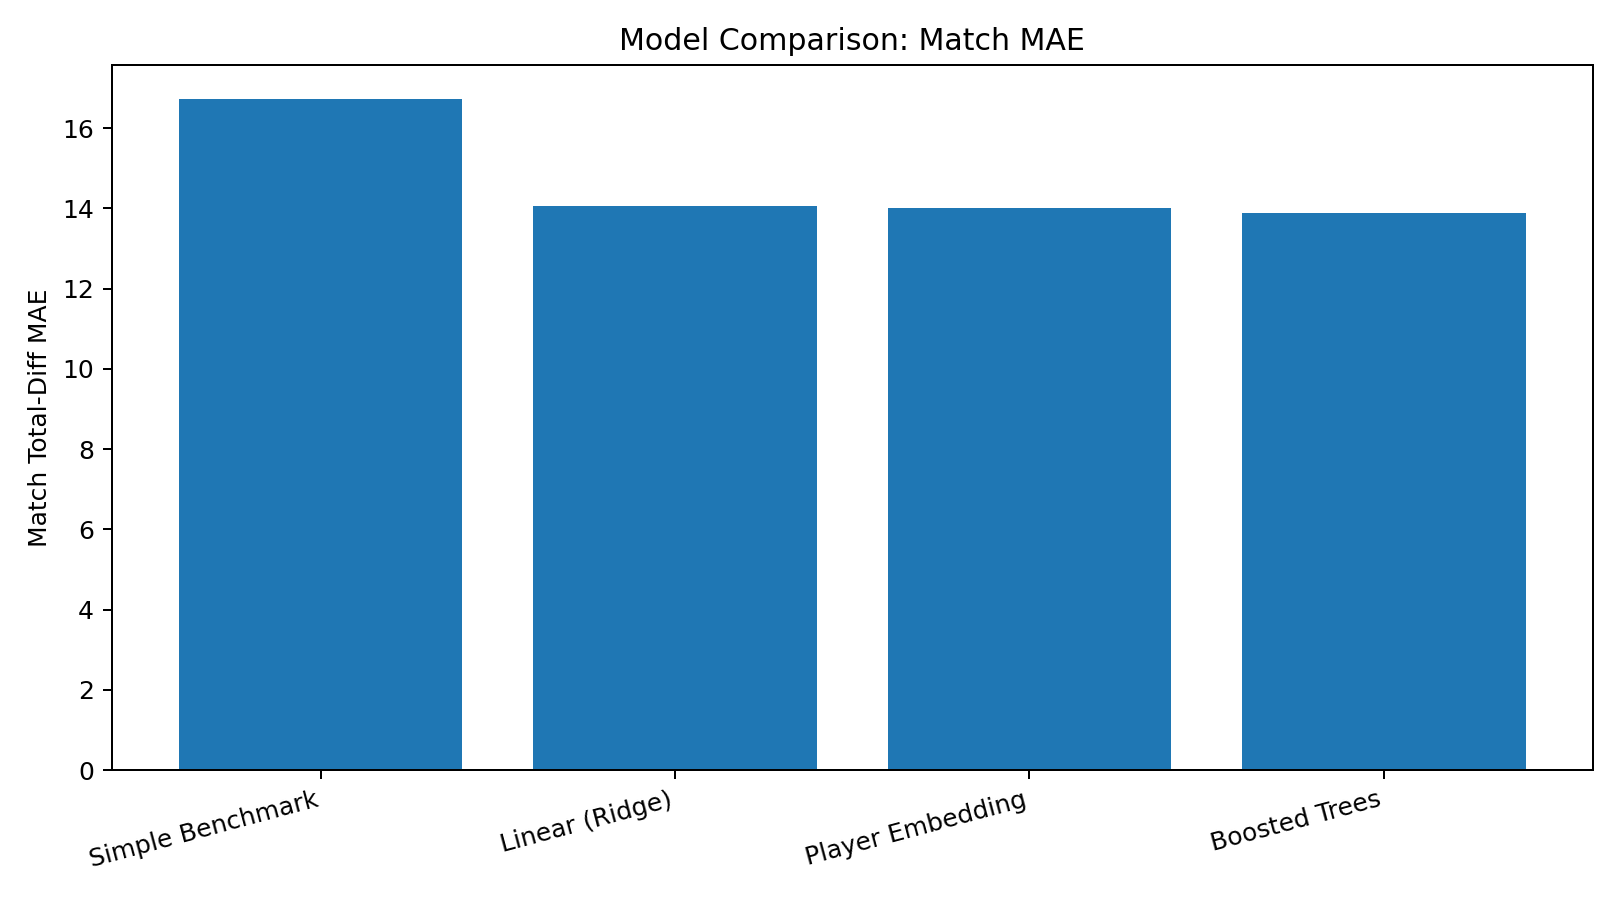
\includegraphics[width=0.92\columnwidth]{figures/model_comparison_mae.png}
    \caption{Comparison of match-level mean absolute error across models. Lower is better.}
    \label{fig:model_mae}
\end{figure}

\begin{figure}[H]
    \centering
    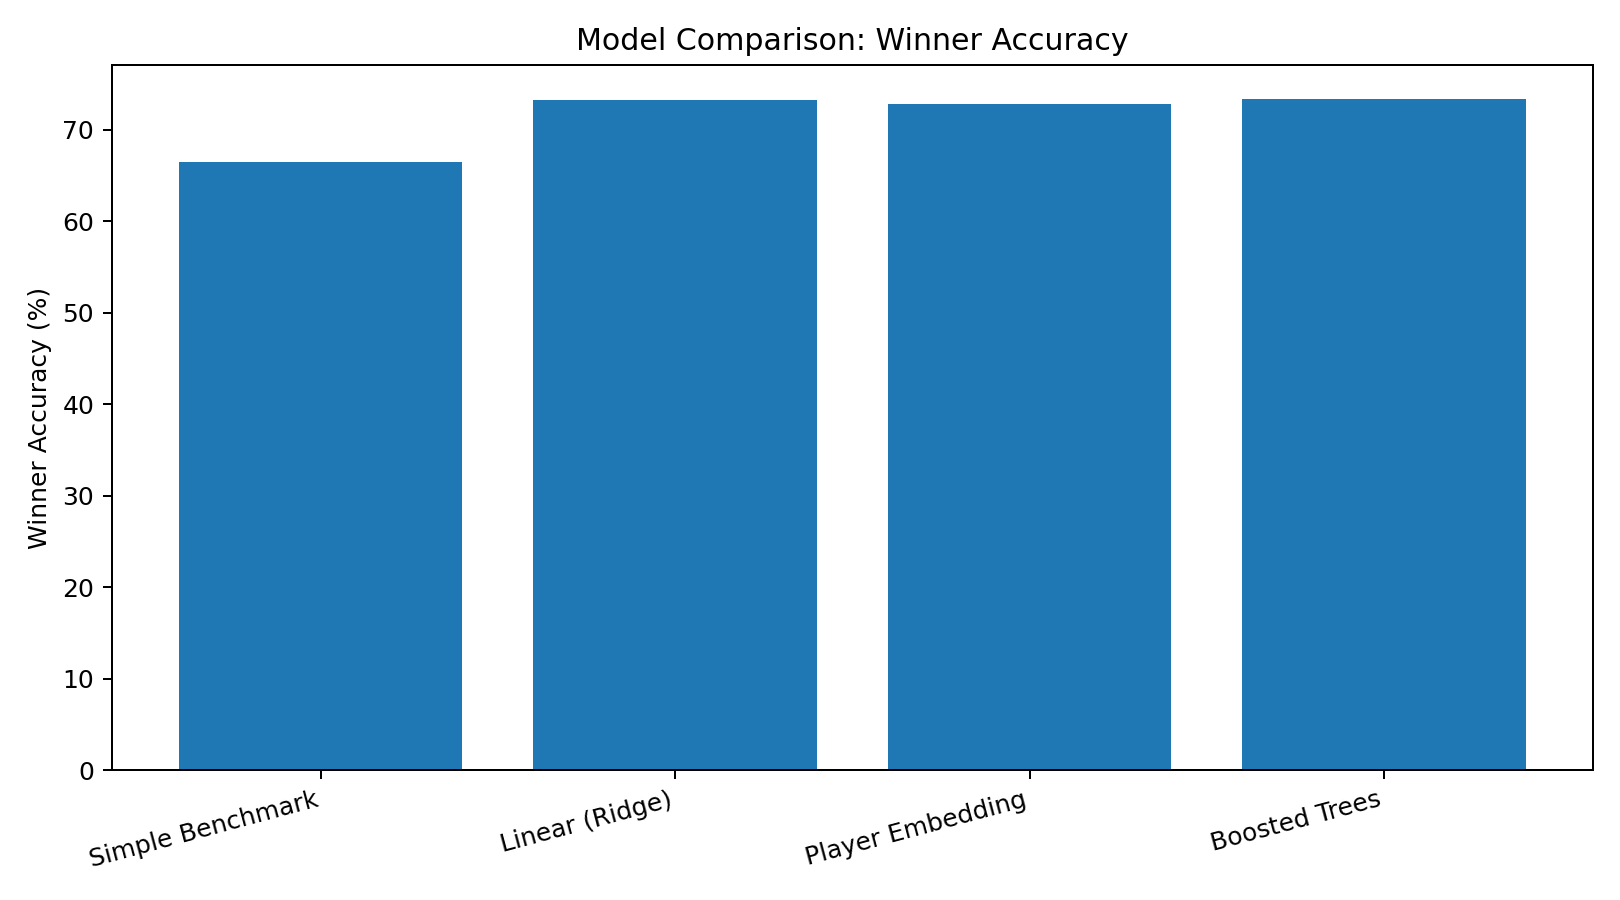
\includegraphics[width=0.92\columnwidth]{figures/model_comparison_accuracy.png}
    \caption{Comparison of winner prediction accuracy across models. Higher is better.}
    \label{fig:model_acc}
\end{figure}

These plots reveal the central empirical pattern of the project. The baseline is meaningfully weaker than all feature-based approaches. Moving from the baseline to ridge regression yields the largest improvement, both in MAE and in winner accuracy. By contrast, the embedding model and boosted-tree model improve only slightly over the linear model. This strongly suggests that the majority of predictive signal is already captured by the engineered features themselves.

Figure~\ref{fig:importance} further supports this conclusion. The most important features in the boosted-tree system are dominated by rating-based signals and related structured statistics, indicating that the dynamic rating model contributes heavily to final predictive performance.

\begin{figure}[H]
    \centering
    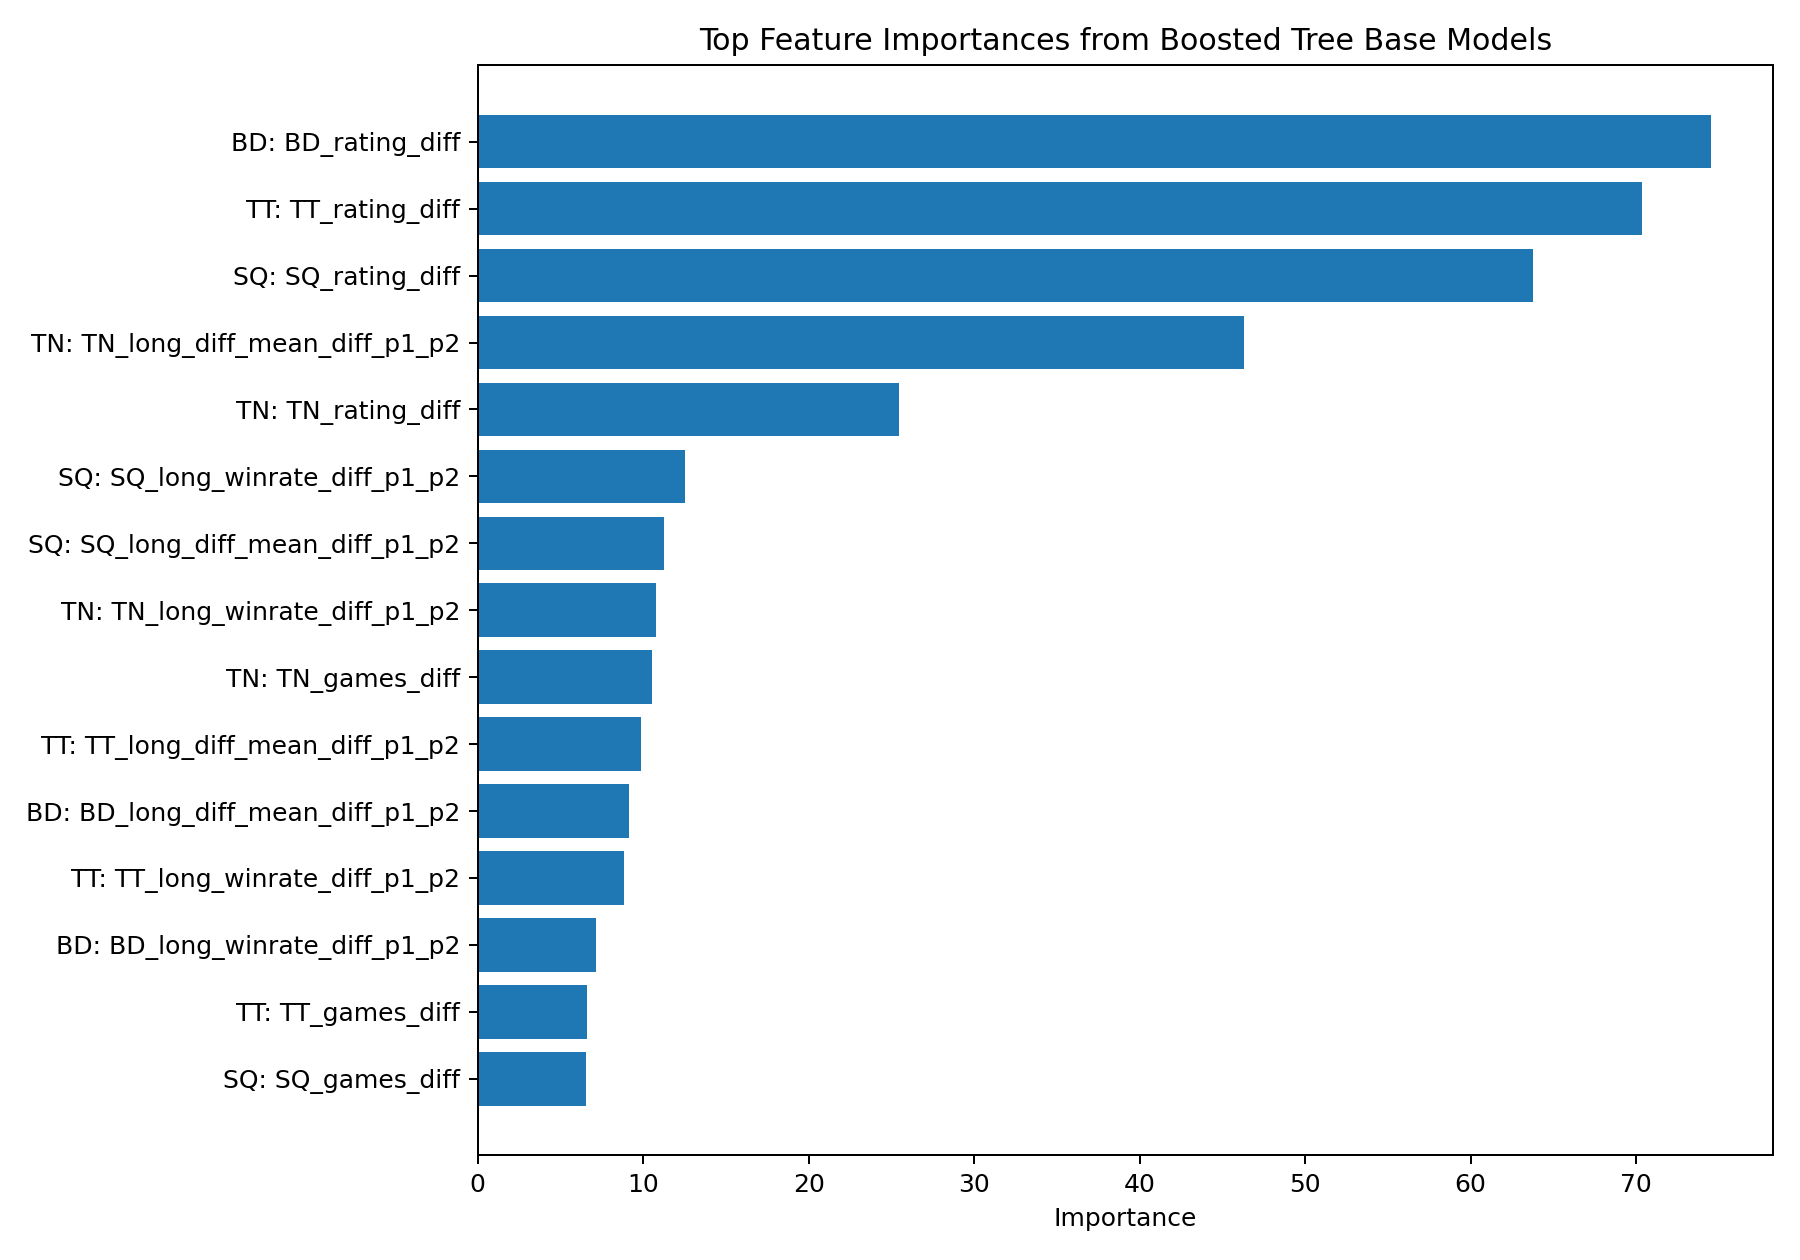
\includegraphics[width=0.92\columnwidth]{figures/feature_importance.png}
    \caption{Top feature importances from the boosted-tree model.}
    \label{fig:importance}
\end{figure}

% =========================================================
\section{Discussion}

The most important conclusion of the project is that representation design dominates model complexity. The single largest improvement occurs when moving from a historical-average baseline to a feature-based linear model. This indicates that once domain-specific information such as rating gaps, recent form, residual behavior, and head-to-head context is encoded explicitly, a large fraction of the prediction problem becomes linearly accessible.

This also explains why the embedding model does not significantly outperform ridge regression. In many machine learning settings, learned latent representations are valuable because the raw input representation is insufficient. Here, however, the handcrafted feature set is already strong and grounded in domain structure. As a result, the embedding model has relatively little new structure to discover.

The same logic applies to boosted trees. They do outperform the other approaches, but only marginally. This does not mean nonlinear models are unhelpful. Rather, it means that the feature space already contains substantial nonlinear structure. The rating system is itself nonlinear through the tanh mapping from rating difference to score difference. Recent residual features measure deviations from nonlinear expectation. Head-to-head features inject interaction-specific corrections. Consequently, even a linear model is operating on inputs that already reflect important nonlinear transformations.

One useful way to summarize the result is:
\begin{quote}
    \emph{Skill differences scale linearly, but outcomes do not; however, once that nonlinearity is explicitly encoded in features, the additional benefit of more flexible models becomes smaller.}
\end{quote}

This insight is valuable beyond the specific application. In structured tabular prediction problems, there is often a temptation to escalate model complexity before fully exploiting problem structure. The results here suggest the opposite workflow: first invest in a representation that respects the mechanics of the problem, then evaluate whether model complexity is still the bottleneck.

Finally, the difference between margin prediction and winner prediction is itself informative. Winner accuracy is materially higher than exact score-difference accuracy, which is expected because sign prediction is a coarser task. This suggests that the system is better suited for identifying likely winners than for forecasting exact match margins with high precision.

% =========================================================
\section{Conclusion}

This project developed a complete pipeline for Racketlon match prediction, beginning with historical data collection and cleaning, continuing through leakage-safe feature construction and sport-specific rating estimation, and ending with multiple predictive models and deployable inference functionality.

The core contribution is not just a single predictive model, but an analysis of where performance actually comes from. Across all experiments, the dominant finding is that feature engineering provides most of the predictive power. The dynamic rating system, recent-form summaries, residual features, long-term aggregates, and head-to-head statistics together create a rich representation of player skill and matchup context. Once that representation is in place, relatively simple models already perform well.

More complex models are still useful. The boosted-tree system achieves the best results overall and captures interaction effects that simpler models miss. However, the size of this gain is limited, which is itself an important scientific result. It shows that in this application, the primary challenge is not lack of model flexibility but designing a feature space that reflects the true structure of the sport.

Future work could extend the system in several directions. Additional contextual variables such as tournament level, location, or recency weighting may further improve predictions. More specialized uncertainty estimation methods could provide better confidence measures than simple geometric neighborhoods. A richer treatment of sequential dependence across sports may also improve match-level realism. Nonetheless, the present results already demonstrate that a principled combination of domain knowledge and machine learning can produce a strong and interpretable sports prediction system.

% =========================================================
\bibliographystyle{plainnat}
\begin{thebibliography}{99}

    \bibitem{elo1978}
    Arpad E. Elo.
    \newblock \emph{The Rating of Chessplayers, Past and Present}.
    \newblock Arco Publishing, 1978.

    \bibitem{friedman2001}
    Jerome H. Friedman.
    \newblock Greedy function approximation: a gradient boosting machine.
    \newblock \emph{Annals of Statistics}, 29(5):1189--1232, 2001.

    \bibitem{chen2016xgboost}
    Tianqi Chen and Carlos Guestrin.
    \newblock XGBoost: A scalable tree boosting system.
    \newblock In \emph{Proceedings of the 22nd ACM SIGKDD International Conference on Knowledge Discovery and Data Mining}, pages 785--794, 2016.

    \bibitem{ke2017lightgbm}
    Guolin Ke, Qi Meng, Thomas Finley, Taifeng Wang, Wei Chen, Weidong Ma, Qiwei Ye, and Tie-Yan Liu.
    \newblock LightGBM: A highly efficient gradient boosting decision tree.
    \newblock In \emph{Advances in Neural Information Processing Systems}, 2017.

    \bibitem{koren2009matrix}
    Yehuda Koren, Robert Bell, and Chris Volinsky.
    \newblock Matrix factorization techniques for recommender systems.
    \newblock \emph{Computer}, 42(8):30--37, 2009.

    \bibitem{mikolov2013word2vec}
    Tomas Mikolov, Ilya Sutskever, Kai Chen, Greg Corrado, and Jeffrey Dean.
    \newblock Distributed representations of words and phrases and their compositionality.
    \newblock In \emph{Advances in Neural Information Processing Systems}, 2013.

    \bibitem{cover1967}
    Thomas Cover and Peter Hart.
    \newblock Nearest neighbor pattern classification.
    \newblock \emph{IEEE Transactions on Information Theory}, 13(1):21--27, 1967.

    \bibitem{bentley1975}
    Jon L. Bentley.
    \newblock Multidimensional binary search trees used for associative searching.
    \newblock \emph{Communications of the ACM}, 18(9):509--517, 1975.

\end{thebibliography}

\clearpage
\appendix

% =========================================================
\section{Appendix}
\subsection{Exploratory Confidence Analysis}

As a secondary experiment, I investigated whether local geometric structure in feature space could provide a proxy for confidence. The idea was that if a test match lies in a dense region of feature space, or if its nearby historical neighbors have highly consistent outcomes, then predictions in that region might be more reliable.

To test this, matchups were embedded into a low-dimensional engineered feature space and indexed with a KD-tree. For each test point, the $k$ nearest training neighbors were queried, and local statistics such as mean neighbor distance and variance of neighbor targets were computed. These statistics were transformed into heuristic confidence measures.

This experiment was informative, but not especially successful. The relationship between simple geometric confidence and actual prediction error was weak. The main reason is likely representational mismatch: the final boosted-tree predictor operates in a richer nonlinear space than what is captured by Euclidean geometry in the selected feature subset. Thus, geometric closeness in the hand-chosen KD-tree space is not necessarily aligned with predictive similarity under the final model.

The confidence analysis is therefore best interpreted as a useful negative result. It shows that uncertainty estimation for nonlinear tabular predictors is not easily solved by simple local-density heuristics.

\begin{figure}[H]
    \centering
    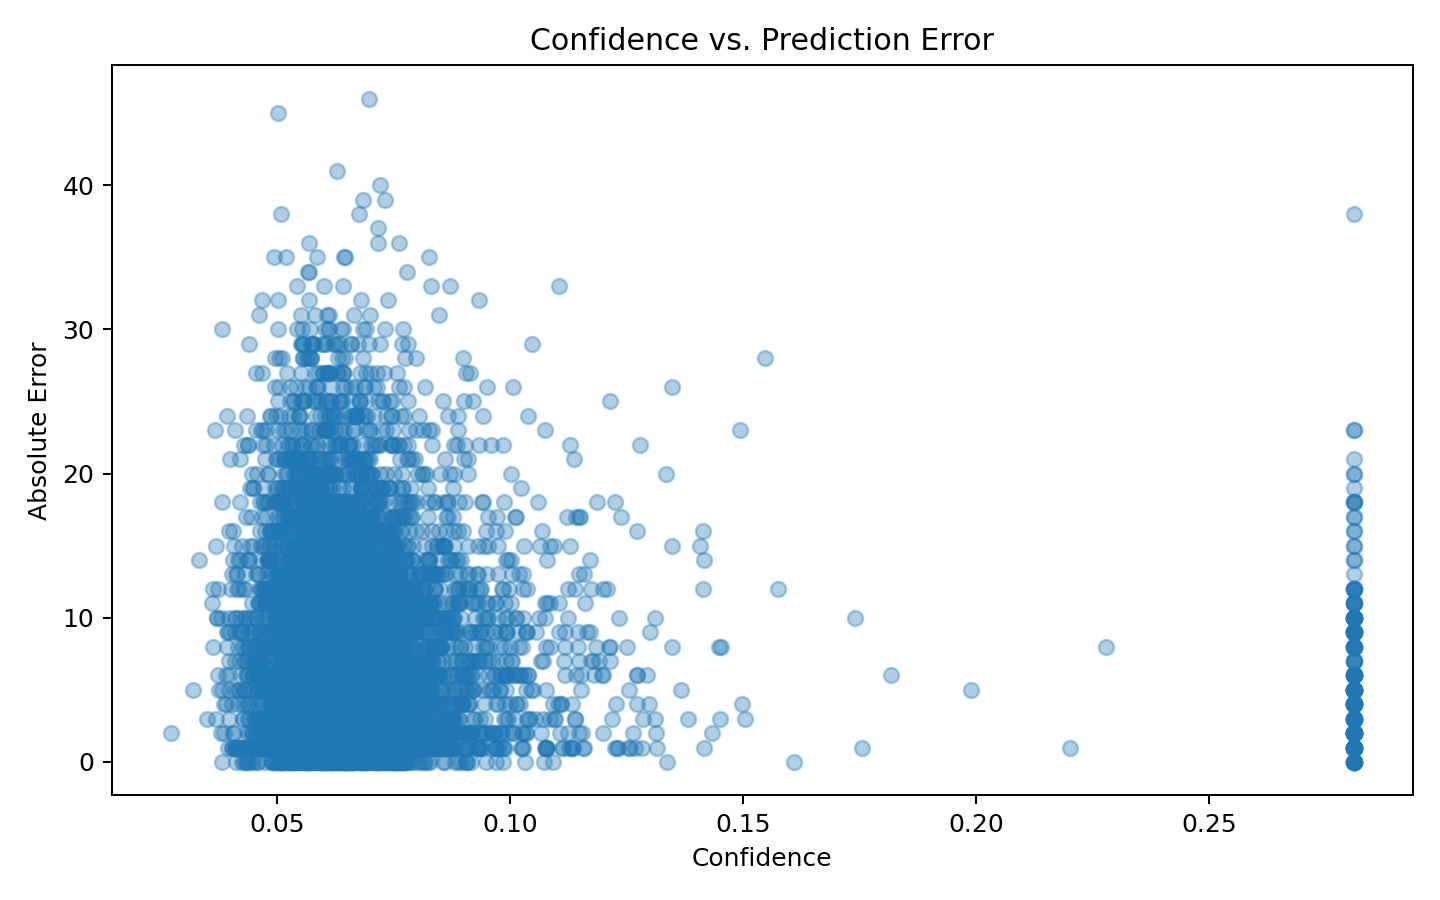
\includegraphics[width=0.9\columnwidth]{figures/confidence_vs_error.png}
    \caption{Relationship between geometric confidence and absolute prediction error.}
\end{figure}

\begin{figure}[H]
    \centering
    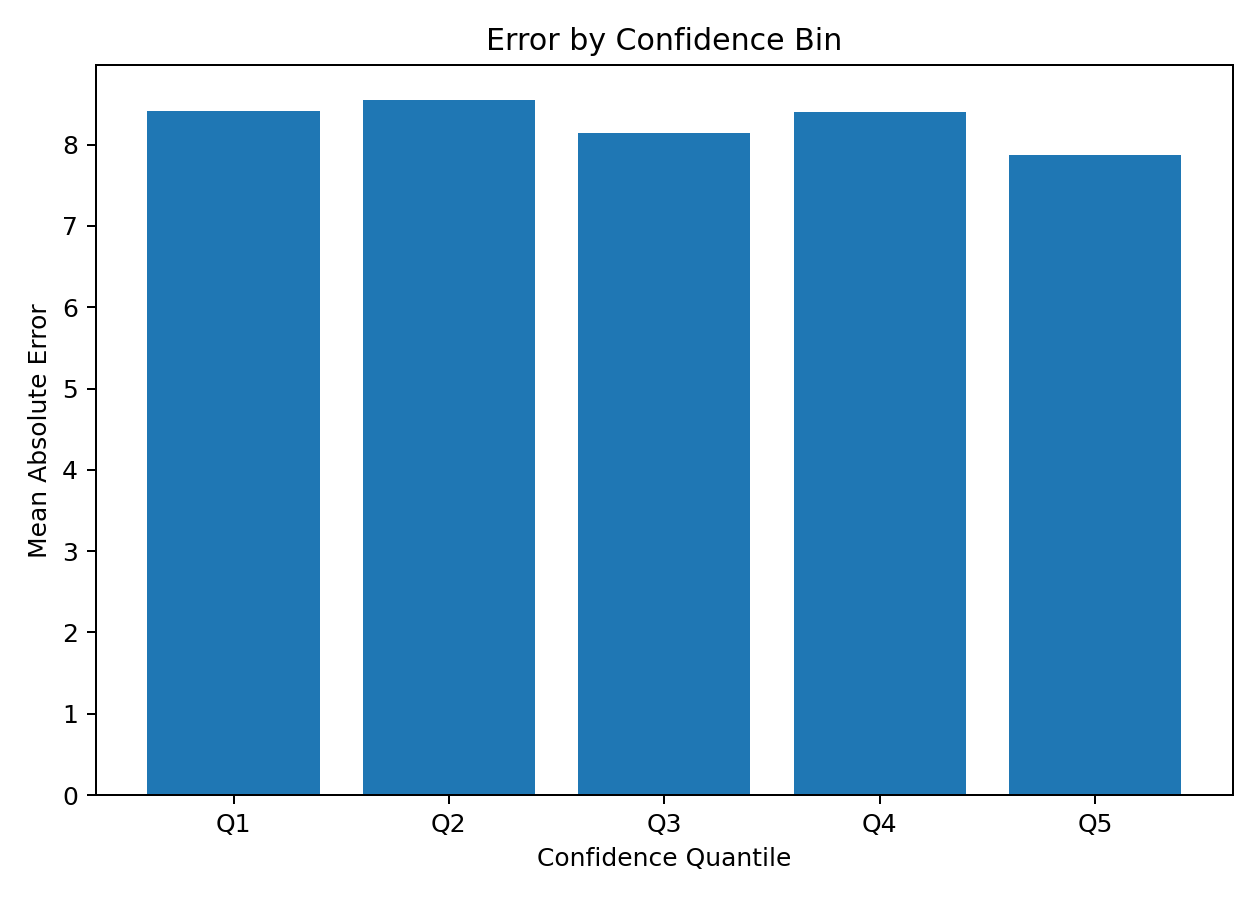
\includegraphics[width=0.9\columnwidth]{figures/confidence_bins_mae.png}
    \caption{Mean absolute error grouped by confidence quantile.}
\end{figure}

% =========================================================
\subsection{Reproducibility Notes}

The full pipeline can be reproduced from four main stages:
\begin{enumerate}[leftmargin=1.2em,itemsep=0.25em]
    \item scrape raw historical match data,
    \item clean and normalize match records,
    \item build chronological feature tables and inference state,
    \item train and evaluate models on the resulting dataset.
\end{enumerate}

The final system also includes a saved inference package capable of synthesizing future matchup features from player names and returning predicted sport-level and match-level outcomes.

For reproducibility, the complete implementation is available at:
\url{https://github.com/ZainMI/racketlon-predictor-and-ratings}.

\end{document}